\documentclass[12pt,a4paper]{article}
\usepackage{geometry}
\usepackage{indentfirst}
\usepackage[english]{babel}
\usepackage[utf8x]{inputenc}
\usepackage{amsmath}
\usepackage{mathtools}
\usepackage{amsfonts}
\usepackage{graphicx}
\usepackage{subfigure}
\graphicspath{ {images/} }
\usepackage[colorinlistoftodos]{todonotes}
\geometry{margin=2.5cm, top = 0.8cm, headheight=80pt,includeheadfoot}
%settting for implement java code------------------------------------------
\usepackage{listings}
\usepackage{color}
\usepackage{courier}

\definecolor{dkgreen}{rgb}{0,0.6,0}
\definecolor{gray}{rgb}{0.5,0.5,0.5}
\definecolor{mauve}{rgb}{0.58,0,0.82}

\lstset{frame=tb,
  language=Java,
  aboveskip=3mm,
  belowskip=3mm,
  showstringspaces=false,
  columns=flexible,
  basicstyle={\small\ttfamily},
  numbers=none,
  numberstyle=\tiny\color{gray},
  keywordstyle=\color{blue},
  commentstyle=\color{dkgreen},
  stringstyle=\color{mauve},
  breaklines=true,
  breakatwhitespace=true,
  tabsize=3
}

\usepackage{fancyhdr}
\pagestyle{fancy}
\usepackage{xcolor}
\usepackage{lipsum}
\fancyhf{}
\lhead{
\includegraphics[width=1.3cm]{figures/X}}
\rhead{
\includegraphics[width=3.5cm]{figures/logo-quantcube_small}}
\fancyfoot[R]{\thepage}
\fancypagestyle{plain}{%
    \renewcommand{\headrulewidth}{0pt}%
    \fancyhf{}%
    \fancyfoot[R]{\thepage}%
}
%-------------------------------------------------------------------
\begin{document}

\begin{titlepage}

\newcommand{\HRule}{\rule{\linewidth}{0.5mm}} % Defines a new command for the horizontal lines, change thickness here

% \center % Center everything on the page
 
%----------------------------------------------------------------------------------------
%	COVER SECTIONS
%----------------------------------------------------------------------------------------


\includegraphics[scale=0.2]{figures/X_logo.jpg} 

Ecole Polytechnique

Master 1 Data Science, 2016/2017 

\large DESHKO Nataliia \\[1cm]

\begin{center}
\textsc{\LARGE RAPPORT DE STAGE DE RECHERCHE}\\[1cm]

\textsc{\Large \textbf{Construction of Sentiment Index in Russian}} \\[1cm] 
\textsc{\LARGE NON CONFIDENTIEL}\\[3.5cm]
\end{center}

Département d’informatique

INF 591 : Informatique

Directeur de stage : Olivier Bournez

Maitre de stage : Thanh-Long Huynh

3 April 2017 - 11 August 2017

QuantCube Technology

19 rue Poissonnière, Paris
\end{titlepage}

%----------------------------------------------------------------------------------------
\large \textbf{Abstract} \\[0.1cm] % https://www.thecipherbrief.com/article/indicators-political-instability-1091

The objective of this research internship is to construct the Sentiment Index in Russian in order to estimate political stability in Russia and Ukraine in real time using publicly available data from Twitter blogs. Work on the introduced topic includes : collecting data (tweets which speak about Russian president Vladimir Putin) for analysis, building the database, filtering, preprocessing, modeling and index calculation.

For natural language processing part I used such techniques as Tf-Idf indicator and Word2vec word representation, for machine learning part - decision trees, boosting algorithms, linear classifiers and neural network were applied as well as distant supervision, which is supposed to adjust neural network for sentiment analysis purposes but did not practically increase the result. The best accuracy score obtained is 0.71.

% Talking about the sources of valuable data, as soon as influence of media is persistently increasing and people are used to share their opinion in the blogs and social networks, the population may benefit from availability of this information.
\newpage
\tableofcontents
\newpage
%----------------------------------------------------------------------------------------

\newpage
\section{Introduction}

Political disruption like military takeover, civil wars and total state disintegration are arduous to predict but have tremendous consequences for State security and the well-being of a population. Therefore, accessing the real-time political state of the country is an object for exploration and might be advantageous for safety, tourism, trade, international affairs etc. Talking about the sources of valuable data, use of media is persistently increasing and people are constantly sharing their opinion in blogs and social networks. The objective of this research internship is to benefit from this fact in order to access political stability in Russia in real time using data from Twitter social network (blogs). Except for being used in economical, humanitarian and safety purposes, political stability index is also a product which ministries of foreign affairs may use for the purpose of predicting risks for the country's residents and travelers abroad in order to better organize their reversion if needed. One more reason for exploring this topic is that it may give deeper insight into economic growth of the country or building the macro-economical index. In general, such indexes are valuable for investors and are widely used in investment strategies for estimating risks and exploring current market state.
%%%%%%%%%%%%%%%%%%%%%%%%%%%%%%%%%%%%%%%
First stage of the Sentiment Index creation represents choosing and collecting data (tweets) for analysis. These tweets are then labeled according to their sentiment to build a train data set. Then, an adapted preprocessing should be applied to the text data. A series of models will then be tested for estimating the sentiment of validation tweets. Their scores will be used to chose the best-performing classification model. After obtaining the most accurate classifier, it is used to predict the sentiment of the test data in real time. These predictions are finally aggregated and used to build a Sentiment index.

The main considered topics are NLP, Database management and Machine Learning, and neural networks in particular.
\newpage

\section{Sentiment index for the political stability}

\subsection{How to define political stability}
Political stability is the ability of a state to survive external shocks \cite{polit_stab}. A State, however, is not a fixed entity : governments, presidents and even dictators can succeed each other without creating political instability. Therefore, it is necessary to identify the factors which determine that a country was affected by a shock. The classical approach in the analysis of political stability is to predict military conflict [10]. According to the Center of Systemic Peace, instability is linked to events such as civil wars, unfavorable regime changes \footnote{The delinquency of a state, the passage from a democracy to an authoritarian regime or the replacement of a non democratic system by a regime that is more repressive} and genocides or politicides \footnote{The murder of members of a certain political faction or other violent acts occurred with the goal of eliminating or neutralizing the activity of the faction.} [12]. However, other types of events can also be a source of political instability. This is particularly the case of the transition from dictatorships to more democratic regimes, as it was the case during the Arab Spring. In addition, considering only the three cases mentioned above is somewhat restrictive, since this kind of events is very unlikely in more developed countries, with a consolidated democracy. This is not to say that political instability does not exist in such countries. For those, the premature termination of a democratically elected government in favor of the opposition, in the respect of the constitution, can also be regarded as a case where the government has not survived a shock.

\subsection{Definition of Sentiment Index}
A graphical or numerical indicator aimed to show how a society feels about the market, business environment or a public figure, for example, is called a sentiment Index. A sentiment indicator attempts to evaluate how various factors such as the political environment, unemployment, inflation or macroeconomic conditions will behave in future. Investors can benefit from sentiment indicators by watching the dynamics of how optimistic or pessimistic people are to ongoing political/market conditions. For instance, companies are less likely to stock up on inventory in case if a consumer sentiment index is displaying the negative attitude, because they are not expecting consumers to spend their budget. \footnote{http://www.investopedia.com/terms/s/sentimentindicator.asp}

\section{Sentiment analysis}
\subsection{Overview}
The rising popularity of Internet blogs and social media is producing huge volume of data. This provides information about people’s opinions on different events, news, and political figures. However, it cannot be manually processed due to its size. Therefore, we are automatizing this task using machine learning, in particular natural language processing. Doing so, we will face up several problems.

Looking at some numbers, just on Twitter 500 million public messages are shared every day. But we should understand that the majority of Internet users (73,7\%) are not English speakers and 66\% of tweets are written in languages other than English. Every language defines its own grammar, vocabulary and syntactic rules. It has become an issue to overcome as soon as multilingual content leads to using several languages at the same time during analysis.

Machine learning approaches such as neural networks provide diverse methods for feature engineering. However, they require a broad set of training data, and this fact becomes a hold-up for the progress in such tasks as classification and prediction. The main difficulty in using global social media data is that the number of trained samples is very limited, depends on language and is quite expensive and time-consuming to get them. This is especially the case for other languages than English, as most research on this topic concerns English language media – annotated corpora, sentiment dictionaries and benchmark datasets are mostly developed for English \cite{SemEval2017}.

Automatic sentiment analysis is a basic issue in NLP (natural language processing). Despite the fact that the evolutions are being constantly made towards this goal, usage of irony, sarcasm, informal language with dialect and specific constructions in human language may easily confuse sentiment classifiers and make the programmed sentiment analysis to be a challenge for machine learning. As well, contextualization takes place on social media and creates an additional complicating factors.  

\subsection{State of art. SemEval}
The best results which exist now for Semantic Analysis of tweets were obtained during Semeval (particularly in 2016 and 2017). SemEval (stands for Sentiment Evaluation) is a competition, goal of which is to improve existing computational semantic analysis systems or develop new ones.

The most recently published research which has outperformed other solutions was presented by J.Deriu, A.Lucchi, V.De Luca, A.Severyn, S.Muller, M.Cieliebak, T.Hofmann, M.Jaggi \cite{SemEval2017} as their solution to SemEval-2016 for the task 4 - sentiment prediction benchmark. Random forest was taken as a baseline method for tweets classification, and the best result archived was obtained using convolutional neural networks (CNN).

The crucial component of their algorithm is a multilayer convolutional neural network (CNN), trained in three phases \cite{SemEval2017}: i) unsupervised, where word embeddings are built on a large corpus of unlabeled tweets (an unsupervised neural language model); ii) distant supervised phase, where the network is learning a weakly-labeled dataset \footnote{In these case it means that a tweet with smileys like ':)' will be weakly-classified as positive and the one like ':(' – as negative. More details on distant supersision and weak labels are specified in the following paragraph} of tweets containing emoticons ; and iii) supervised phase, during which manually annotated tweets are used to train the network . This system has gained an F1-score of 62.7\% on the English test data of SemEval-2016 \cite{SemEval2015}

While existing convolutional approaches \cite{sent2015} permit to take any language for training, these still require a sufficient amount of training data. We aim at the solutions which do not expect us to maintain manual labeling for every new language needed, and here is a couple of them proposed: (1) automatically translation the data into English and running the existing classifier in English - this option belongs to transfer learning approach \footnote{ Transfer learning allows us to deal with scenarios when no or little labeled data is provided by leveraging the already existing labeled data of some related task or domain.} or (2) train a CNN using only weakly-labeled tweets without using any supervised data. Evidently, a fully-trained CNN is expected to perform better than the foregoing cases. On the other hand, it is unclear if such an improvement would be significant and will provide an excuse for manual labeling of thousands of tweets.

\subsubsection{Weak labels, distant supervision}
For various tasks, specific heuristics and existing datasets may play a role of the weak supervision. \cite{weakSup} These indicators are 'features' of data. When we need training data for application of machine learning techniques, there are diverse ways to automatically do it using existing databases, rules-of-thumb, heuristics, etc. Employing such features is called a weak supervision because it might contain some inaccurate or even contradicting, conflicting data, so cannot be used instead of supervised set. But after some refining it may be applied effectively.

Weak supervision datasets might have such origins:
\begin{itemize}
\item Ground-truth data which is available but is not an exact match for the current task, however, is close enough to be useful (usually called a "distant supervision")
\item Domain heuristics (e.g. common patterns, rules of thumb, etc.)
\item Biased or "weak" classifiers
\item Irregular non-expert annotators (crowdsourcing, for instance)
\end{itemize}

Firstly, a large corpus or a prepared neural language model is used to initialize word embeddings. Then, a distant semi-supervised or unsupervised corpus of tweets is used by convolutional neural network to train them. Later, its parameters are tuned by training CNN on the supervised dataset.\cite{sent2015} 

This approach has been actively explored lately in machine learning and diverse NLP applications in particular. \cite{SemEval2017} Unsupervised training is empirically proved to be beneficial for supervised machine learning tasks \cite{benj_pretr}. In the mentioned paper, authors considered an option of distant pre-training which is represented by inferring weak labels from data without manual classification. The task of text polarity classification was fulfilled with this algorithm, using the notably larger training sets gathered from texts containing smileys ( authors of \cite{techn_rep_stanf} have got accuracy above 80\%). In \cite{sent2015_UNITN} Severyn and Moschitti have presented that training a CNN on datasets with emoticons with further supervised training on a smaller set of manually annotated labels boosts the performance of the described algorithm.

\subsubsection{Word2vec model as a word embedding for NLP}
Word2Vec \cite{w2v_model} is a model producing a vector representation of words from a corpus of texts. The particularity of this representation is that the distribution of vectors in the space depends on their meaning. Words with close meanings will be close according to the notion of the cosine similarity. The vector operations' properties are also applicable here: for example, Mikolov and Dean \cite{mikolov_dean} have discovered that the resultant vector of the operation "Paris -France + Italy" is close to the vector "Rome". Using this representation of the words contained in the tweets, we hope to be able to take into account the proximity of words and perform better than with a representation which deals with the synonyms of any kind.

The construction of such a model requires training a shallow neural network. Its task is to predict the 2k words \textit{$w_{t−k}$, $w_{t−k+1}$, ..., $w_{t−1}$, $w_{t+1}$, ..., $w_{t+k}$} surrounding the word $w_{t}$ in the corpus. Consider a corpus with a vocabulary of size $|X|$. This vocabulary is indexed by the integers \textit{0, 1, ..., $|X|$ − 1}. The model that we are interested in takes as an input a word, represented as a vector-column of size $|X|$ consisting of ones on the row corresponding to its index and 0 elsewhere (one-hot encoding). It then projects this word into a space of low dimension using a projection matrix P. Finally, the word representation in this new space will be used to calculate the probability of occurrence for the 2k words neighbors (Figure \ref{fig:skip_gram}). For j ∈ \textit{\{−k, −k + 1, ..., -1, 1, ..., k − 1, k\}}, this probability is estimated as follows:
\[\mathbb{P} (w_j \vert w_t) = \frac{\exp{({v^T_{w_j}} u^T_{w_t})}}{\sum_{w=1}^V \exp{V^T_{w_j}}u^T_{w_t}}\]
Where \textit{u} is the original representation of the word and \textit{v} the one in the space of smaller dimension.

The issue here is to obtain the projection matrix P so that the prediction of the neighbors of $w_{t}$ is the best possible. For any initial representation \textit{u} and final \textit{v}, we have $u^{T}P = v$. The representation of "one-hot vector" of vectors in the initial space means that \textit{P} is in fact the transpose of the concatenation of the vectors representing the words in the final space. Thus, to get this matrix, we maximize the log likelihood average :
\[\frac{1}{T} \sum_{t=1}^T \sum_{-k\leq j\leq k} \log p (w_{t+j} \vert w_t)\]

We would therefore consider the gradient of this function. However, the size of the vocabulary makes this computation prohibitive. Optimization methods and proxies for the softmax are presented in \cite{mikolov_dean}.

In the current case, the model appears to place the words with the similar meaning close to each other. We note that the token which is the word "power" in Russian without the ending, is close (within the meaning of the cosine similarity) to tokens associated with words or hashtags which consider to the government, parliamentarian parties and corruption (see Figure \ref{fig:simil_vlast}).
\newline
\begin{figure}
\centering
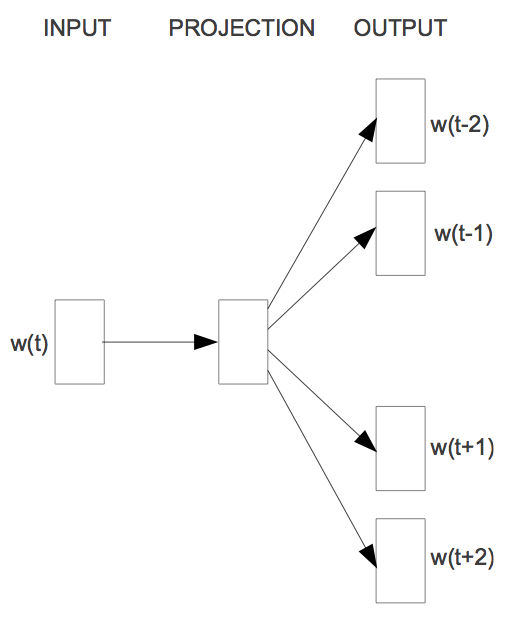
\includegraphics[width=0.3\textwidth]{figures/skip-gram.png}
\caption{Skip-gram model}
\label{fig:skip_gram}
\end{figure}
\newline
\begin{figure}
\centering
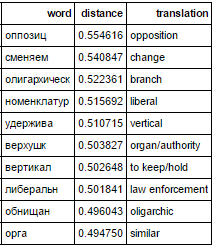
\includegraphics[width=0.3\textwidth]{figures/simil_vlast.PNG}
\caption{Word2vec word similarity}
\label{fig:simil_vlast}
\end{figure}

\subsubsection{State of art: Sentiment Analysis in Russian}
What about research made distinctly for Russian language, there are several papers which consider sentiment analysis in Russian \cite{blinov}, \cite{chetviorkin}, \cite{panchenko} (and, particularly, within the framework of Russian Information Retrieval Seminar ROMIP). One of them observes Russian speaking Facebook and conducts general analysis of the emotional level of the social network (measures 'happiness', in other words) as well as presents the distribution of the sentiment along the time \cite{panchenko}. However, it doesn't observe sentiment index, calculated for a specific object. It is worth to notice, that according to the results in \cite{panchenko} positive posts are more frequent then negative ones on Russian-speaking Facebook, which is not the case for the political posts in Twitter that will be depicted in the following sections.

One of the points of view shown in the papers presents lexical approach, which implies creation of the emotional dictionary and relies on it during texts sentiment estimation. This way is quite complicated, significantly relies on the domain and doesn't generalize well \cite{blinov}, \cite{panchenko}.

%There also exist an engine for defining the sentiment of the texts, including the sentiment which relates to some object. http://eurekaengine.ru/ru/demo/


\newpage

\section{Implementation}
As a main part of my internship I started by developing Sentiment Index for political popularity of Russian president and continuing with conducting analysis of politics in Ukraine. In the following document I will describe what was performed and what results were obtained for the first part.

\subsection{Collecting data}
Among current most popular social networks such as Twitter, Vk \footnote{Vk is a Russian social network, analogical to Facebook. As statistics claim, 80 million users are using VK every day, from https://vk.com/page-47200925\_44240810. According to my observations, VK is more used for entertainment, than for sharing opinion on politics, market etc},  Facebook \footnote{Facebook counts 13.1 million of Russian users as for Sept, 2016, from http://expandedramblings.com/index.php/russian-social-media-stats-yandex-vkontakte/} Twitter is widely used for opinion mining as soon as messages posted by its users are short, informative and frequent. In addition to that, Twitter service provides API for accessing its data programmatically. Thus, it was chosen for my work as a source of data.

\subsubsection{Twitter and API}
Twitter is an on-line news social networking service where users post and interact with messages, "tweets", restricted to 140 characters. After Twitter was created in March 2006 and launched in July, the service rapidly gained worldwide popularity. In 2012, more than 100 million users posted 340 million tweets a day, and the service handled an average of 1.6 billion search queries per day. In 2013, it was one of the ten most-visited websites and has been described as "the SMS of the Internet". As of 2016, Twitter had more than 319 million monthly active users. On the day of the 2016 U.S. presidential election, Twitter proved to be the largest source of breaking news, with 40 million election-related tweets sent by 10 p.m. (Eastern Time) that day. \footnote{https://ru.wikipedia.org/wiki/Twitter}

Twitter provides programmatic access to read and write Twitter data with use of its API. For my goal I was using The Streaming API which provides developers with the low latency access to Twitter’s global stream of Tweet data. Messages which indicate the events that have occurred, will be pushed to a streaming client. \footnote{https://dev.twitter.com/streaming/overview}

\subsubsection{Choosing and collecting relevant data}
As soon as we are interested in political stability in Russia, and the language spoken there is Russian, the first filter applied is the language of the tweet. Than, we should take into account that we are looking for the tweets which somehow mention Putin. With the help of Stream API, which allows to perform search by keywords, we can extract the tweets needed.
Next, we have to take into account that Russian language is used not only in Russia, but also in Ukraine, Belarus, Kazakhstan and other countries, that is why additional filters should be implemented.

When saving the tweet, we deal with tweet object, it contains not only username and text of the tweet, but also public user profile details (profile description, date of profile creation, location, timezone, number of followers etc.) and time of the status (tweet) publication, number of 'retweets', likes etc. Despite the fact that the location field is ofter empty or contains inappropriate string, it may give some information together with profile's description.
I have gathered names of all the Russian cities, towns and regions in Russian and English into one list and was comparing its elements to the location specified in the tweet author profile. Then, I was using such a criteria: 
\begin{itemize}
\item if location is empty, or it is not empty and is contained in the list specified above, tweet gets label 'from Russia'
\item if location is not in the list, we look into profile description and if it contains '+7' (phone code in Russia) or '.ru' (Internet domain), the tweets is classified to be from Russia
\item otherwise the post is labeled as 'not from Russia'
\end{itemize}

In order to collect tweets in real time with Twitter API, its PHP interface was used. I have modified the script, provided by the company, so that I can use it for my purposes.

\subsubsection{Sentiment labels}
In order to build sentiment index for V.Putin, we need to access the population's attitude to him. In this work we will make such conclusions relying in the tweets, so at first what should be done is preparing learning sample by hand so that the algorithm could learn, namely, there should be labels manually put on the sampled posts. Main labels that were used are:
\begin{itemize}
\item 0 - negative (the person doesn't like Putin/considers him to be bad politician/wouldn't vote for him at the elections)
\item 1 - neutral (plain facts and mentions with no sentiment, opinion or attitude are classified to this group)
\item 2 - positive (the person likes Putin/appreciates what he does/would vote for him at the elections)
\end{itemize}

One more additional label (4) is applied to the tweets which are not relevant. They were not considered during learning because they may affect it and make the results more noisy.

I have labeled distinctive 2,098 tweets, which will be used in the future for machine learning.
\newline
\begin{figure}
\centering
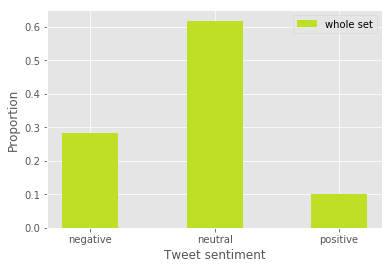
\includegraphics[width=0.8\textwidth]{figures/label_distr.png}
\caption{Distribution of labeled tweets over sentiment}
\label{fig:label_distr}
\end{figure}

Distribution of labels from the learning sample according to the sentiment is shown on Figure \ref{fig:label_distr}. As we may see, labels are not distributed uniformly, and there is a bias towards negative sentiment. We will have to consider this fact in future, in particular during choosing an evaluation score and putting labels for the incoming tweets.

% \subsubsection{Saving collected tweets}
Data collection should be carried out constantly. 
% In current work MySQL database system is used and contains several tables/views for storing:
% \begin{itemize}
% \item all of the tweets with labels 'from Russia' or 'not from Russia'
% \item tweets with sentiment labels
% \item tweets to classify
% \end{itemize}

% Tables with tweets consist of such columns:
% \begin{itemize}
% \item date of tweet
% \item text of tweet
% \item username
% \item location
% \item links
% \item timezone
% \item description
% \item from Russia label
% \item sentiment label
% \end{itemize}
Once we have the data for the analysis, we are proceeding with Python.

\subsubsection{Tweets distribution}
Let's look how tweets are distributed over time - with daily and hourly peaks - shown on Figures \ref{fig:all_distr_month_day}-\ref{fig:dist_hour}.
\begin{figure}
\centering
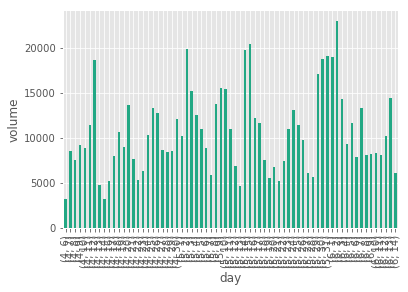
\includegraphics[width=0.8\textwidth]{figures/all_distr_month_day.png}
\caption{Distribution of relevant tweets over time, grouped by month and day}
\label{fig:all_distr_month_day}
\end{figure}
\begin{figure}
\centering
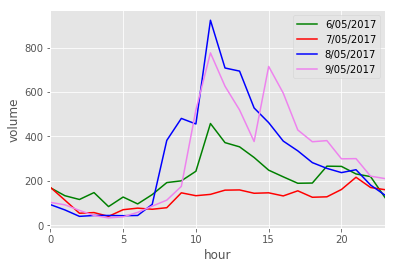
\includegraphics[width=0.6\textwidth]{figures/distr_hour.png}
\caption{Example of hourly distribution of tweets}
\label{fig:dist_hour}
\end{figure}
% \begin{figure}
% \centering
% 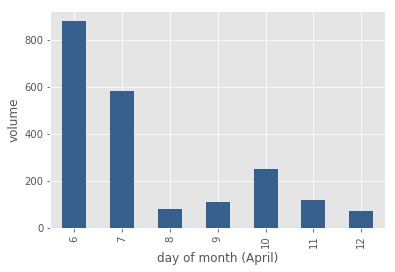
\includegraphics[width=0.6\textwidth]{figures/labeled_data_distr_day.png}
% \caption{Distribution of relevant tweets over time, grouped by day}
% \label{fig:labeled_data_distr_day}
% \end{figure}

We may also take a look at the number of original and reposted tweets (see Figure \ref{fig:all_distr_retweets}). Number of 'retweets' is significant, and using this fact will make future predictive algorithm less time-consuming.
\begin{figure}
\centering
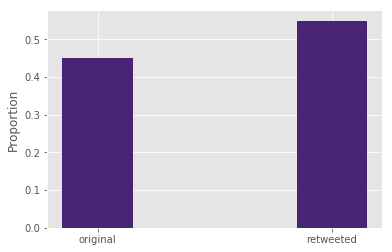
\includegraphics[width=0.6\textwidth]{figures/all_distr_retweets.png}
\caption{Distribution of tweets by originality}
\label{fig:all_distr_retweets}
\end{figure}

After gathering data into a database, we have 2,098 items in the table with labeled tweets and about 736,000 records in the table which contains all of the relevant posts and is being populated permanently. For comparison, there are  tweets in the general table which also keeps tweets with 'not from Russia' label. The proportions are shown on Figure \ref{fig:distr_from_russia}. As we may notice, minor part of tweets is not from Russia but it is still essential to filter them out because sentiments of the opinions shared in and outside the country might be opposite, and so, in order to avoid biased index we have to make selection according to the location.
\newline
\begin{figure}
\centering
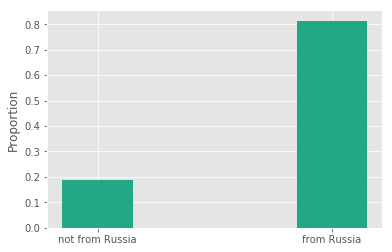
\includegraphics[width=0.6\textwidth]{figures/distr_from_russia.png}
\caption{Distribution of all collected tweets over location}
\label{fig:distr_from_russia}
\end{figure}
\newpage

\subsection{Preprocessing}

Preprocessing consists of:
\begin{enumerate}
\item Removing targets (mentioning of other users in the beginning of the post) - they may disturb during classification.
\item Removing links - they will no be helpful for learning.
\item Dropping duplicates - we don't need them during learning but should take into account every incoming tweet (in particular, duplicates) while index calculation.
\item Sentences tokenization - so that we could work with words in sentences but not the whole sentences.
\item Stopwords removal (optional)
\item Stemming (optional)
\end{enumerate}
\newpage

\subsection{Feature engineering}
Baseline feature engineering is represented by Tf-Idf (stands for term-frequency - inverse document frequency) bag-of-words which represents short for term frequency–inverse document frequency. It is a numerical statistic that is supposed to reflect how important a word is to a document in a collection or corpus.

However, it is logically to admit that the words by themselves don't manage to fully grasp the sentiment. So I proceeded with vector representation of words implemented by Word2vec (gensim module in Python).

First attempt was done by creating word representations \footnote{word representations are used to build a sentence representation which will be finally used. Sentence representation is computed as a vector mean of its words' representations} based on my own database - texts of all the tweets.  However, my database is not big enough yet (vocabulary contains 13,129 words) to have enough of learning material. That is why next attempts of using word2vec were also compared with utilization of the ready vector representation, calculated from other datasets. The biggest one (which was finally selected) represents the corpus trained on Wikipedia using fastText and contains 1,888,423 tokens. These vectors of dimension 300 were obtained using the skip-gram model described in Bojanowski et al. (2016) with default parameters \cite{w2v_model_wiki}. This set performed the best, and that is why will it be used as a vector representation for words in our tweets and referenced in future as a corpus. In addition, different options for text preprocessing (such as stemming and stop words removal) were examined and the results will be presented in the following part.

\newpage

\subsection{Choosing a metric}
The metrics which may be used:
\begin{itemize}
\item accuracy
\item Precision which is the fraction of relevant instances among the retrieved instances
\item Recall which represents the fraction of relevant instances that have been retrieved over total relevant instances 
\item F1 score, it is a measure of a test's accuracy and is calculated as a weighted average of the precision and recall: \[ 2  \frac{precision * recall}{precision + recall}\]
\end{itemize}

Since we have multi-label classification task, the way of treating these scores for each class should be chosen. As was shown on \ref{fig:label_distr}, proportions of tweets volume differs with their sentiment, and the neutral dominate. We have to take it into account while evaluating the predicting models - they will tend to produce more neutral labels, and there will be a lot of true positives among them, which will unreasonably boost the score (because we are interested in positives and negatives). Therefore, we have to pay attention more to the prediction capacity for the labels with the sentiment. That is why it is more efficient to build the scorer based exclusively on positive and negative labels.

With F1 score we can access a more realistic measure of the classifier's performance. Moreover, we will not be mislead, for example, in case of poor precision and high recall (which is the situation when all of the documents are classified as positive) which in average will give an intermediate score. As for accuracy score, it will be mostly influenced by the neutral values, and so it is not very demonstrative either.
As mentioned, recall and precision individually do not capture the quality of the predictions completely. In contrast, F1 takes into account both of them and will be considered to be the best indicator. But we have a set with 3 unique labels so F1 score calculation needs averaging. Mean of F1 scores for positives and negatives is chosen as a scorer for  cross-validation while selecting a model. The same as for the accuracy, F1 score lie in the interval [0;1] and 1 represents the best quality of predictions. 

\subsection{Choosing a model}

Train/test samples are respectively 50,3\% and 49,7\%.

Once data is prepared and features are defined, we are moving on to the prediction model.

If we try to pick the predictions randomly (one from 3 classes), the accuracy is about 33\% with the F1 averaged for positive and negatives about 23\%. The baseline accuracy, calculated on Tf-Idf features using simple RandomForestClassifier with 50 estimators is 0.636 (averaged F1 for positive and negatives is 0.36).

Among various machine learning techniques such ones were taken into consideration and examined for different parameters using cross validation:
\begin{itemize}
\item Boosting algorithms: AdaBoost, Gradient Boosting
\item Decision trees: Random Forest, Extra Trees
\item Support vector machines (SVM)
\item Linear classifiers: Logistic Regression with L1 and L2 regularization
\item Neural Networks
\end{itemize}

Each model was fitted with various set of its specific parameters (using Random Search), evaluated using cross validation and further compared between each other. 

Scores using features by TfIdf are presented on Figure \ref{fig:tfidf} .
\newline
\begin{figure}
\centering
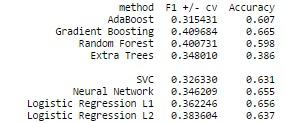
\includegraphics[width=0.6\textwidth]{figures/results_tfidf.jpg}
\caption{Results using Tf-Idf features}
\label{fig:tfidf}
\end{figure}

Results of the mentioned techniques, applied to data represented by Word2vec, are displayed on Figure \ref{fig:w2v}-\ref{fig:w2v_wiki_nostem_noswr} with different options for feature generation and preprocessing like stop words removal and application of stemming during preprocessing.

\begin{figure}
\centering
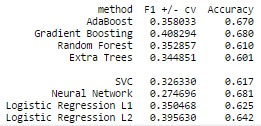
\includegraphics[width=0.6\textwidth]{figures/results_w2v.jpg}
\caption{Results using Word2vec model based on OWN database WITH stop words removal and stemming}
\label{fig:w2v}
\end{figure}

\begin{figure}
\centering
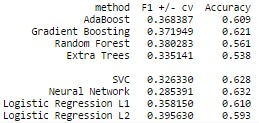
\includegraphics[width=0.6\textwidth]{figures/results_w2v_nostem_noswr.jpg}
\caption{Results using Word2vec model based on OWN database WITHOUT stop words removal and stemming}
\label{fig:w2v_nostem_noswr}
\end{figure}

\begin{figure}
\centering
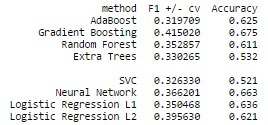
\includegraphics[width=0.6\textwidth]{figures/results_w2v_wiki.jpg}
\caption {Results using Word2vec WIKI model WITH stop words removal and stemming}
\label{fig:w2v_wiki}
\end{figure}

\begin{figure}
\centering
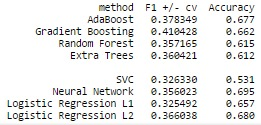
\includegraphics[width=0.6\textwidth]{figures/results_w2v_wiki_nostem_noswr.jpg}
\caption{Results using Word2vec model based on WIKI database WITHOUT stop words removal and stemming}
\label{fig:w2v_wiki_nostem_noswr}
\end{figure}

After examining classical methods I was using 1D convolutional neural network \footnote{http://www.wildml.com/2015/11/understanding-convolutional-neural-networks-for-nlp/} (see example of CNN on Figure \ref{fig:cnn}) implemented in keras for further improvements of the results. 

\begin{figure}
\centering
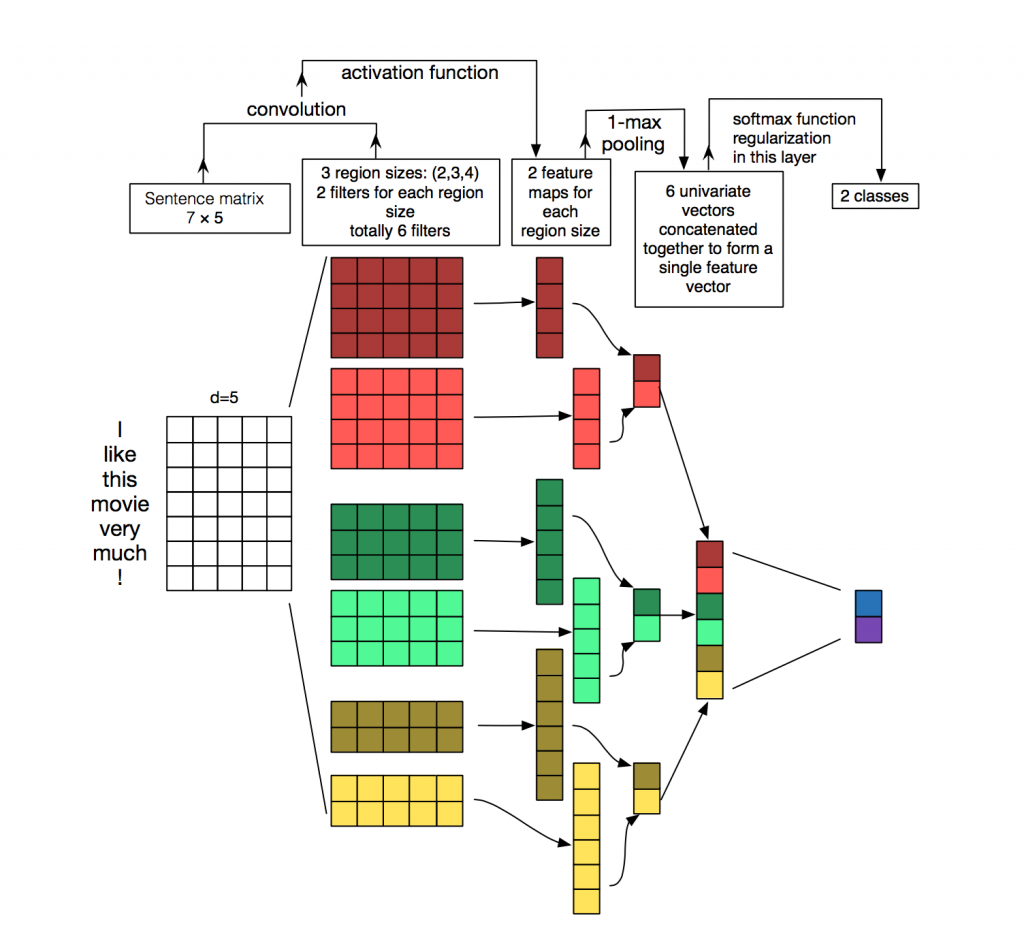
\includegraphics[width=1\textwidth]{figures/cnn.png}
\caption{Illustration of a Convolutional Neural Network (CNN) architecture for sentence classification. Here  three filter region sizes are depicted: 2, 3 and 4, each of which has 2 filters. }
\label{fig:cnn}
\end{figure}

\subsubsection{CNN architecture}
Adjusting the architecture to the current purposes provides such settings:
\begin{itemize}
\item Categorical crossentropy was taken as a loss (as soon as we have multiple labels). 
\item In order to prevent overfitting and catch the moment of the best trade off of train and validation loss, early stopping technique is provided, and it monitors validation loss. So, if the model will not improve the score for a definite number of epochs (for 30 epochs in the current case) the learning will be stopped.
\item There is one more technique applied against overfitting - dropout (a regularization technique for reducing overfitting in neural networks by preventing complex co-adaptations on training data)
\end{itemize}

\begin{figure}
\centering
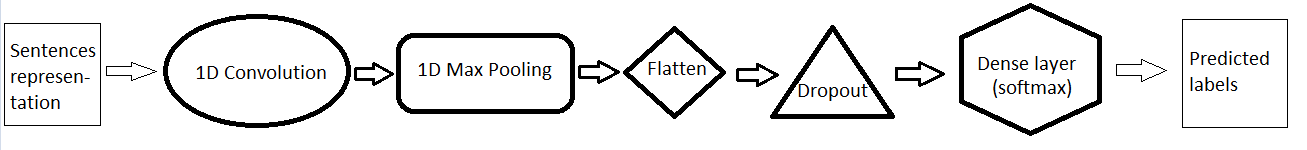
\includegraphics[width=1\textwidth]{figures/cnn_arch.PNG}
\caption{Architecture of convolutional NN}
\label{fig:cnn_arch}
\end{figure}

The final architecture (see Figure \ref{fig:cnn_arch} ) includes one convolutional layer with same padding, ReLU activation, and window size is equal 5; pooling layer (max-pool), flattening layer, dropout, and a dense layer with softmax activation. For the optimization, Adam optimizer is taken. 

Parameters which were tuned for CNN:
\begin{itemize}
\item Learning rate, the most influential variable 
\item Number of filters in the convolution
\item Kernel size (the length of the 1D convolution window)
\item Padding (padding for a sliding window)
\item Activation (a function of a node which defines the output of the node given an input or set of inputs)
\item Pool size (size of the max pooling windows)
\item Dropout rate
\end{itemize}

The network used is not deep (1 layer), that is why change of the parameters other than learning rate did not make significant change during their tuning.

Here word embeddings are initialized by Wiki neural model, both trainable/not trainable setting were examined (trainable means that the weights will be updated during training). As we see, the results are not really different. Scores (for one of the cases/folds of cross-validation) are shown in Figure \ref{fig:results_cnn_nottr}-\ref{fig:results_cnn_tr} together with error and training error, accuracy and training accuracy plotted (it should be noticed that some variation takes place, that is why final scores, which will be mentioned, were obtained using 5-fold cross-validation).

\begin{figure}
\centering
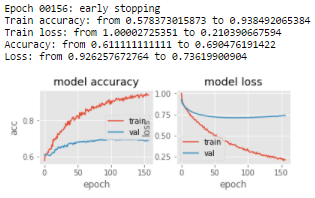
\includegraphics[width=0.5\textwidth]{figures/results_cnn_nottr.PNG}
\caption{Result obtained using Word2vec WIKI model, 1-layer CNN, non-trainable embedding}
\label{fig:results_cnn_nottr}
\end{figure}

\begin{figure}
\centering
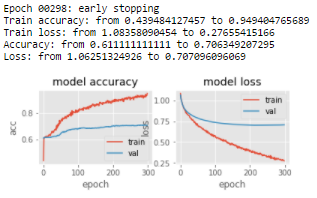
\includegraphics[width=0.5\textwidth]{figures/results_cnn_tr.PNG}
\caption{Result obtained using Word2vec WIKI model, 1-layer CNN, trainable embedding}
\label{fig:results_cnn_tr}
\end{figure}

After doing 5-fold cross-validation for the current networks we have such scores (they have slightly improved from the previous models):
\begin{itemize}
\item Non-trainable: Accuracy = 0.67897, F1 (+-) =  0.4012
\item Trainable: Accuracy = 0.70933, F1 (+-) =  0.45464
\end{itemize}

% \begin{figure}
% \centering
% 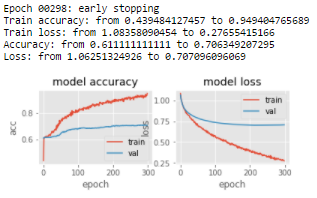
\includegraphics[width=0.5\textwidth]{figures/results_cnn_tr.PNG}
% \caption{Results using Word2vec WIKI model, 1-layer LSTM network, trainable embedding}
% \label{fig:results_lstm}
% \end{figure}

% \begin{figure}
% \centering
% 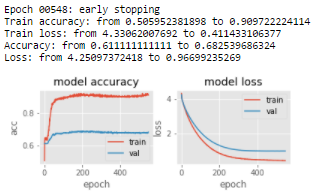
\includegraphics[width=0.5\textwidth]{figures/results_cnn_lstm_tr.PNG}
% \caption{Results using Word2vec WIKI model,1-layer CNN + 1-layer LSTM network, trainable embedding}
% \label{fig:results_cnn_lstm}
% \end{figure}

As we may see, keras NN didn't appear to significantly improve the last result. Likely, neural network would perform better with more training data.

\subsubsection{Distant learning}
Next step concerns unsupervised tuning the NN with weak labels, or weak sentiment. The database is being populated with tweets in Russian which contain at least one of 90 smileys, and which are classified according to the sentiment of the smiley. Feeding this data to a network before classified data may help it to learn the specifics of the dataset but requires a considerable volume of information to learn on.

My database of emojies at the moment contains about 623,000 tweets. After being collected they are assigned weak labels: if a tweet contains positive/negative smiley, it is given the corresponding label; in case when items from both classes are presented in a tweet, it is supposed to be neutral. After looking into the database and cleaning the set from noise and plotting the distribution we may see (Figure \ref{fig:smileys_distr}) that there is a bias towards positive tweets - they are significantly dominating.
\newline
\begin{figure}
\centering
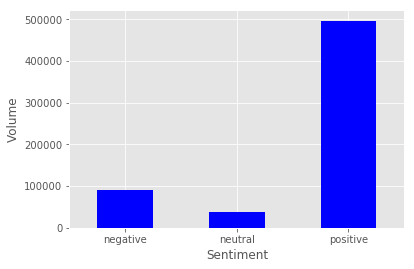
\includegraphics[width=0.8\textwidth]{figures/smileys_distr.PNG}
\caption{Distribution of smileys data sentiment}
\label{fig:smileys_distr}
\end{figure}

Now, we will use the CNN with the same structure as before, but firstly we fit it on unsupervised data set (for several epochs and with low learning rate so that the network didn't learn closely), and after this, when weights are somewhat adjusted to the data with sentiment, the network is learning on the supervised (labeled) set (in our case, for 2000 epoch or until the early stopping).

After tuning the parameters and executing the code with unsupervised and supervised sets, the result which was gained by cross validated CNN using distant learning, is represented by accuracy = 0.69722, F1 (+-) =  0.44198 (averaged for positive and negative classes).

Plots and results for one of the tests (folds of cross-validation) are presented on Figure \ref{fig:results_cnn_dist}.
\newline
\begin{figure}
\centering
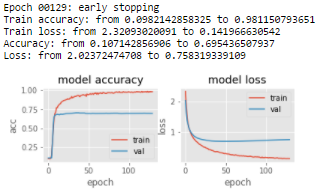
\includegraphics[width=0.5\textwidth]{figures/results_cnn_dist.PNG}
\caption{Results by CNN with distant learning using weak "smiley" labels}
\label{fig:results_cnn_dist}
\end{figure}

Unfortunately, the quality of prediction didn't increase. It means that distant learning currently is not useful. There may be several explanations for such a result:
\begin{itemize}
\item  the first guess could be that tweets which concern politics, together with their true sentiment are too specific. People express their feelings using irony very ofter, while tweets collected for distant supervision are quite primitive in this sense - they contain positive emoticons if the author likes something and negative in the opposite case. They might be suitable for exploration of the public opinion on some goods, movies etc, when people are more straightforward in their publications. So, finally, non-typical structure of tweets about Putin caused the predictions, made with weak labels to be too noisy.
\item other option, which is also quite probable, is that the volume of weak labeled data is not sufficient. Other researcher mentioned in their papers that they used over 1 million datasets, so it would be interesting to look what happens with more samples and see if better word representations (for the current topic) are obtained.
\item However, there is still at least one more possible explanation for a weak performance, and it is about optimization. There might be ways to boost the score just modifying the architecture and further tuning the parameters.
\end{itemize}

Finally, CNN claimed to be the best prediction model. Its cross-validated accuracy on the training set of 2016 items is about 0.71 and F1 score as average of positive and negative labels (computed the same as earlier) is 0.45. Thus, it is taken for further consideration.

\subsection{Index calculation}
Once we have a classification model, the data, which is constantly incoming with the tweets, may be classified into positive, negative and neutral classes. Then, knowing hourly volume of each class we are computing the Sentiment Index with the following formula: 
\[idx_{hourly} = \frac{1}{2} (\frac{pos - neg}{pos + neg} +  1) \] where \textit{pos} is number of positive tweets for the preceding hour and \textit{neg} - number of negatives. 
Using this formula we will always obtain an absolute value from the interval [0;1], with sentiment being completely negative at 0 (only negative tweets observed) and completely positive at 1 (there are only positive posts and no negative ones).

Index values are displayed at the company's portal in the row with other indexes (of politics, crude oil, trades etc) for different countries.

\section{Conclusion}
During my internship at first I was learning articles which represent current state of art of sentiment analysis of the media and suggest different solutions for various cases. The major part of the research results I was using, was done in the framework of SemEval competitions during several last years. The task of computing sentiment for popular topics has been popularized with the increasing number of Internet users and public discussions in the networks. However, the gained accuracy is still not perfect and requires refining, and we face such main problems as the different styles of opinion expression and difficulties of natural language processing, in particular, of the informal language which may contain sarcasm, irony and hide the context that is not explicitly mentioned. 
As a partial result of my research internship the Sentiment Index for Russian president Vladimir Putin, based on the Russian Twitter media, was developed.

In particular, I have developed the idea of weak learning for Russian which was earlier presented only for English. However, it didn't seem to improve the predicting capability of the classifier (in comparison with the 1D CNN with no distant supervision), probably because of the specifics relative to the structure of tweets about politics.
Not to mention, the model is specifically tuned for the current language (Russian), population's communication habits and topic, and it gained the prediction accuracy of 0,71.

\section{Further research}
In future studies regarding this topic, the network architecture might be refined (in addition to CNN - convolutional neural network consider RNN - recurrent neural network , LSTM - long short time memory neural network, and their combinations) (maybe together with upgraded distant supervision) in order to boost the score of neural network.
One more direction for the further deeper exploration is feature engineering - there might be other new/upgraded competitive word/sentence representations which may allow to look at the data from the different angle and discover significant features. Another active problem concerns unbalanced proportions of labels in training data - this issue also may have some extend for exploration.

In addition, gathering more data (which takes time) may also be advantageous for improving the score. 

Current Sentiment Index can be extended for Ukrainian media and politics but with some new issues:
\begin{itemize}
\item two languages are spoken in Ukraine (Ukrainian and Russian) in approximately equal proportions. Despite the fact the they are similar in some sense, the vocabulary differs, and it means that Ukrainian cannot be processed together with Russian at the same time, but considering tweets of only one of them will make the sample not to be representative.
\item discussions about Ukrainian politics don't go around the only person at the current moment of time, so there is no primitive way to labelize the data. And the more labels there are, the less accurate the model becomes.
\item another concern is about filtering out inappropriate tweets. The baseline is to look for keywords which are discriminative for the relevant tweets using Text Mining techniques.
\end{itemize}

Apart from politics, Sentiment index may also be build (and used) for crude oil and other publicly popular topics in Russia with additional particularity for any applicable subject. Normally, it is interesting to look at how the constructed model will generalize for similar tasks applied to other fields. 

\begin{thebibliography}{9}
\bibitem{SemEval2017} 
Jan Deriu, Aurelien Lucchi, Valeria De Luca, Aliaksei Severyn, Simon Müller, Mark Cieliebak, Thomas Hofmann, Martin Jaggi: Leveraging Large Amounts of Weakly Supervised Data for Multi-Language Sentiment Classification 
\textit{ WWW '17 Proceedings of the 26th International Conference on World Wide Web}. 
Pages 1045-1052. Perth, Australia — April 03 - 07, 2017.

\bibitem{sent2015} 
Aliaksei Severyn, Alessandro Moschitti: Twitter Sentiment Analysis with Deep Convolutional Neural Networks.
\textit{ SIGIR '15 Proceedings of the 38th International ACM SIGIR Conference on Research and Development in Information Retrieval}. Pages 959-962. Santiago, Chile — August 09 - 13, 2015 

\bibitem{sent2015_UNITN}
A. Severyn and A. Moschitti. UNITN: Training Deep Convolutional Neural Network for Twitter Sentiment Classification. 
\textit{ In SemEval 2015 - Proceedings of the 9th International Workshop on Semantic Evaluation}, 2015.

\bibitem{SemEval2015} 
J. Deriu, M. Gonzenbach, F. Uzdilli, A. Lucchi, V. De Luca, and M. Jaggi. Swisscheese at semeval-2016 task 4: Sentiment classification using an ensemble of convolutional neural networks with distant supervision. 
\textit{ Proceedings of SemEval}, pages 1124–1128, 2016.

\bibitem{weakSup} 
Alex Ratner, Stephen Bach, Chris Ré: Data Programming: Machine Learning with Weak Supervision

\textit{$http://hazyresearch.github.io/snorkel/blog/weak_supervision.html$}

\bibitem{w2v_model_wiki} 
P. Bojanowski, E. Grave, A. Joulin, T. Mikolov, Enriching Word Vectors with Subword Information
\textit{arXiv preprint arXiv:1607.04606}. 2016

\bibitem{w2v_model} 
Tomas Mikolov, Ilya Sutskever, Kai Chen, Greg Corrado, Jeffrey Dean: Distributed Representations of Words and Phrases and their Compositionality
\textit{arXiv:1310.4546 [cs.CL]}. 2013

\bibitem{polit_stab} 
Keith M. Dowding and Richard Kimber : The meaning and use of political stability.
\textit{European Journal of Political Research}, 11(3):229–243, 1983.

\bibitem{mikolov_dean} 
T. Mikolov and J. Dean : Distributed representations of words and phrases and their compositionality. 
\textit{Advances in neural information processing systems}, 
2013.

\bibitem{benj_pretr}
D. Erhan, Y. Bengio, A. Courville, P.-A. Manzagol, P. Vincent, and S. Bengio. Why does unsupervised pre-training help deep learning? 
\textit{The Journal of Machine Learning Research}, 11:625–660, 2010.

\bibitem{techn_rep_stanf}
A. Go, R. Bhayani, and L. Huang. Twitter Sentiment Classification using Distant Supervision. 
\textit{Technical report, The Stanford Natural Language Processing Group}, 2009.

\bibitem{blinov}
Blinov P.,  Klekovkina M.,  Kotelnikov E.,  Pestov O.  Research of lexical approach and machine learning methods for sentiment analysis. 
\textit{In Proceedings of Dialog}, Bekasovo, 2013 

\bibitem{panchenko}
A. Panchenko. Sentiment Index of the Russian Speaking Facebook
\textit{Proceedings of the International Conference on Computational Linguistics and Intelligent Technologies "Dialogue"}, Moscow, Russia, 2014

\bibitem{chetviorkin}
Chetviorkin, Ilia, and Natalia Loukachevitch.  Evaluating Sentiment Analysis Systems in Russian. ACL 2013 (2013): 12.

\end{thebibliography}
\end{document}